\documentclass[11pt,a4paper]{article}
\usepackage[utf8x]{inputenc}
\usepackage{ucs}
\usepackage{amsmath}
\usepackage{amsfonts}
\usepackage{amssymb}
\usepackage{url}
\usepackage{graphicx}
\usepackage{subfigure}
\usepackage{fancyvrb}

\newcommand{\question}{\textbf{\\----NEED REVIEW HERE----\\}}


\author{HU, Pili \\
MobiTeC, IE Department, CUHK \\
\texttt{hupili [at] ie [dot] cuhk [dot] edu [dot] hk} \\
\url{http://personal.ie.cuhk.edu.hk/~hpl011/} 
}

\title{Adaptive Video Streaming: 
 \\ a Survey and Case Study}

\begin{document}

\maketitle

\begin{abstract}
	In the past decade, Internet traffic has seen a significant 
	change from web browsing to video viewing. The ongoing trend 
	raises a chanllenging problem: how to stream data to heterogeous 
	peers? 
	
	The designer of such data streaming architecture should 
	bear the following considerations in mind: QoE, server load, 
	network resource efficiency, scalability, etc. The heterogeneous 
	peer network condition makes the design more complicated. The 
	underlying codec ranges from Multi Description Coding to Multi 
	Layer Coding. The data deliver architecture ranges from unicast,
	multicast, to P2P network. Researchers have focused on different 
	system settings and optimization objectives. 
	 
	This paper will first
	sum up several works in the context of adaptive video streaming. 
	At the same time, we do a case study on a commercial adaptive 
	video streaming system, which combines Multilayer Codec and P2P 
	technology. Possible improvements on this system are proposed
	with reasoning. Some of the conjectures are
	verified through a corresponding simulation platform based on NS2. 
\end{abstract}

\pagebreak
\tableofcontents
\pagebreak

\section{Introduction}

\subsection{Background}

\question

\subsection{Paper Structure}
In section(\ref{sec:gen_model}), we propose 5 metrics and 
present a very general model 
of system design as well as several variations. In section(\ref{sec:problem_scope}), 
we propose three problem scopes involved in adaptive video streaming. 
We address the full design from three aspects: codec, networking and playback. 
In section(\ref{sec:p2p_vod}), we focus the networking on p2p technology, 
which is considered a very powerful tool to provide a system with huge 
aggregate bandwidth in a distributed fashion. A design consideration 
list is given from bottom to top. In section(\ref{sec:case}), we do 
a case study on a widely used P2P simulation platform\cite{huang2010simulation}. 
There are not so many highlights from this case study. Nevertheless, 
we conclude some experience in section(\ref{sec:conclusion}), and 
propose some potential directions in section(\ref{sec:future}). 

\section{General Model}
\label{sec:gen_model}

\subsection{Metrics}

No matter what our target system is
(live streaming/Vod; multicast/P2P; layered/or not), we propose 4 general 
system metrics: 
\begin{itemize}
	\item [(QoS)] QoS is one of the traditional considerations. 
	Typical metrics in video streaming is buffer ratio, startup delay, 
	jitter, etc. In \cite{xiao2009layerp2p}, Xiao proposed four metrics 
	in the context of multilayer P2P video streaming: throughput, 
	layer delivery ratio, useless packet ratio, and jitter(subscribe/drop layer 
	events). 
	\item [(QoE)] Note that all systems should benefit their users
	in the first place. However, QoS can not directly reflect user experience. 
	User experience can be measured using Mean Opinion Score\cite{wang2011-perceptual}
	or User Satisfaction Index. The former one is subjective, which involves
	field test on a batch of users. The latter one is objective, which combines 
	several QoS metrics and output one overall score. 
	Current works in adaptive video streaming seldom consider QoE carefully. 
	It's obvious that a QoE aware design is highly appreciated. 
	\item [(Vendor cost)] Cost of system vendor is often considered as 
	the main optimization objective. Some recent VoD works like 
	\cite{wu2011vod-rep} and \cite{zhou2011statistical} fall into this 
	category. In those works, server is modeled as a backup of any missing
	chunks. Thus the QoE(only discontinuity here) is guranteed naturally. 
	With this setting, people can try to lower the server load. 
	\item [(User cost)] User resources, like CPU cycle, network bandwidth, etc, 
	are all precious. If QoE can be guranteed using less resources, it's 
	not a good idea to consume more. Computing resource is prominent if we 
	want to upgrade to a complex strategy. Some strategies look good in model, 
	but may not be applicable due to very high time complexity. For example, 
	in \cite{zhang2006optimal}, Zhang proposed a Mincost Flow based technique, 
	to solve the chunk selection problem. This technique is universal and can 
	solve all similar problems with utility definition. However the time consumption 
	in real deployment is not fully addressed. We believe it consumes 
	more time than the Knapsack based technique proposed in \cite{eberhard2010knapsack}, 
	although the problem definition in the latter work is narrower. In 
	many real deployments, we sacrifice the quality of solution for tractable 
	computation resource. As is given in \cite{eberhard2010knapsack}, an efficient 
	heuristic based algorithm can perform as nearly equally good as the optimal 
	algorithm. In this case, the heuristic basd algorithm may be more likely 
	to be adopted by real system designers. 
	\item [(System cost)] In a P2P system, besides the bandwith consumption at 
	server and peer side, the flow in intermediate netowrk infrastructure 
	should also be taken into consideration. In \cite{chu2001case}, Chu use
	link stress as one of the metrics, which measures how much redundant flow
	tranverse a single physical link. This work is believed to be one of the 
	pioneering work in P2P, so the author considers system cost thoroughly. 
	Later, P2P technology has been proven an efficient method in many real 
	deployments. The following works focus more on client and server side, rather
	than on the network system. 
\end{itemize}

As far as we know, none of the current works consider 
all four metrics in design, although many works can achieve 
good result in those metrics even if they are not considered 
from the very beginning. 

\subsection{Model 1}

One optimization abstraction is:
\begin{eqnarray}
	\text{maximize}&& \text{QoE} \\
	\text{minimize}&& \text{Cost} \nonumber 
\end{eqnarray}

QoE and Cost alone can be multi-dimensional. As is given in last 
section, cost can be categorized into vendor cost, user cost, and 
system cost. Note that this multi-objective model is intractable 
since the two groups of objectives are opposite to each other 
most time. Two simplifications are given in the following section. 

\subsection{Model 1(a)}

By constraining cost to be less than a certain level, 
the original model becomes a single objective optimization. 
$C_0$ can be chosen such that the cost is approximately 
(but not necessarily)
minimum. 

\begin{eqnarray}
	\text{maximize } && \text{QoE} \\
	s.t. && \nonumber\\
	\text{Cost} &\leq& C_0 \nonumber
\end{eqnarray}

This philosophy is widely seen in many works. i.e. set
$C_0$ to be the largest amount of resources available, 
and then optimize QoE(or QoS for simplicity) metrics. 
It is not seen that people constrain resources
(i.e. only use half download bandwidth) when QoE
is not the maximum. 


\subsection{Model 1(b)}

By constraining QoE to be larger than a certain level, 
the original model becomes a single objective optimization. 
$Q_0$ can be chosen such that the QoE is approximately 
(but not necessarily)
maximum. 
\begin{eqnarray}
	\text{minimize } && \text{Cost} \\
	s.t. && \nonumber\\
	\text{QoE} &\geq & Q_0 \nonumber
\end{eqnarray}

This philosophy is widely accepted in the degisn of VoD. 
Zhou proposed a statistical model\cite{zhou2011statistical}
 to analyze the optimial 
replication of VoD. In that work, QoE is guaranteed naturally
by assuming the server as a backup at any time. So the rest
of that work aims at minimizing server load. 


\subsection{Comments on Models}

Theoretical bound deduction is not seen in the scope 
of video streaming, let alone adaptive video streaming. 
In terms of adaptation, we want to know how the tradeoff
between quality sacrifice and other metrics is, given 
certain resources. This is generally Model 1(a), with 
QoE decomposed into several parts. 


\section{Problem Scope}
\label{sec:problem_scope}

We divide the problem from bottom up into three parts:
\begin{itemize}
	\item Codec. It determines how the video is coded, 
	and what kind of adaptation it can have. 
	This is not our research focus. However the 
	choice of codes influences what we can do in the networking
	design. 
	\item Networking. This part solves the problem that how we
	deliver data from server to all receivers efficiently, and 
	meet certain playback requirements at the same time. Most 
	of our work lies in this part. 
	\item Playback. User actions and playback decisions are 
	studied, so that we have a more clear direction when designing 
	networking solutions. Again, this part is not our focus, but 
	gives methodology and tool to facilitate networking design. 
\end{itemize}

\subsection{Codec}

There are two types of adaptive codec:
\begin{itemize}
	\item Multi-Description Coding(MDC). MDC has been studied long ago 
	in the field of information theory\cite{gamal1982achievable}. The basic
	idea is to decompose video data into multiple descriptions. Descriptions
	are independent of each other. With more descriptions received, the 
	receiver can playback higher quality video. For a good survey, interested 
	readers are recommended to \cite{wang2005mdc}. Some application 
	of MDC in video streaming appeared around 2000, to name a few classical 
	works, \cite{apostolopoulos2001reliable}, \cite{apostolopoulos2002multiple}. 
	In \cite{apostolopoulos2002multiple}, Apostolopoulos combines MDC with 
	CDN technology to provide multiple route for video streaming, thus higher
	achieving higher error-resilience. 
	
	\item Multi-Layer Coding(MDC). MLC is different that data is organized 
	layer by layer. Higher layers have dependency on low layers. 
	H.264/SVC\cite{schwarz2007overview-svc} is the extension of 
	H.264/AVC\cite{wiegand2003overview-avc}, which provides three types of 
	scalability: spatial scalability, temporal scalability, and 
	quality scalability. In academic study, temporal scalability is 
	frequently used, for the resultant chunk size is a pyramid look 
	structure. The temporal scalability relys on temporal predictions, 
	in a I-P-B frames fashion. I-frame and P-frame is often put in 
	the base layer, and B-frame forms enhancement layer(s) typically. 
	The typical frame size is: I-frame $>$ P-frame $>$ B-frame. In this case, 
	base layer is usually larger than enhancement layer. In industrial 
	deployment, spatial scalability is more preferred in heterogeneous 
	device distribution. i.e. a cellphone users have smaller screens. 
	There is no incentive for them to download full sized version. 
	If mere temporal scalability is used, they have probably have no choice
	but to download the full sized base layer. The video will not playback 
	smoothly. However, if spatial scalability is used, they can afford 
	the smaller-sized version with better smoothness.  
\end{itemize}

Some important characteristics of the two types of coding 
are summarized in table(\ref{tbl:comp_mdc_mlc}). 
\begin{table}[htb]
\centering
\caption{Comparison of MDC and MLC}
\label{tbl:comp_mdc_mlc}
	\begin{tabular}{c|c|c}
		\hline
		Item & MDC & MLC \\
		\hline
		dependency & independent & dependent \\
		coding efficiency & lower & higher \\
		real deployment & less & more \\
		\hline
	\end{tabular}
\end{table}

Another important consideration of codec is whether 
it's variable bitrate or not:
\begin{itemize}
	\item Variable Bit Rate(VBR) may achieve higher coding 
	efficiency. i.e. when the video is presenting a series of
	consecutive static scenery, it can be coded very efficiently 
	using motion vector compensation. The resultant bit stream 
	may consist of a big I-frame followed by many small P- and 
	B- frames. Observed in time domain, the bitrate is variable. 
	\item Constant Bit Rate(CBR) works at making the bitrate nearly 
	a constant. A common way is to add a feedback buffer to VBR coding
	framework\cite{liu2003adaptive}. The encoder will adjust its 
	quantization level according to buffer status, and make the overall 
	bitrate oscillating around a constant. Two common problems are 
	buffer overflow and buffer downflow. 
\end{itemize}
According to our survey, CBR is commonly used in previous works. This is 
because the constant rate makes system design easier. i.e. in the desgin 
of adaptive video streaming, people always try to prevent jitter
(frequently switch between higher and lower quality). If the codec is
VBR, the receiver may observe a "better bandwidth" when it downloads 
some chunks faster. However, the real reason is the lower video bitrate
during that period of time. If CBR is used, number of chunks downloaded 
in unit time can better reflect the network condition. Thus, better
control over quality adaptation can be achieved. 


\subsection{Networking}

We discuss three types of fundamental networking choices in 
this section: multicast, unicast, P2P. 
In real systems, designers may combine more than one
methods together. i.e. in P2P VoD system desgin, peers can turn to 
server for help. Some systems treat server as a normal peer. This 
simpifies the system and is widely accepted in many studies. However, 
server exihbits much larger capabilities than normal peers. 
Distinguishing the server from normal peers and do some specific optimiztion
may enhance the system. 
In one measurement study of popular online video websites\cite{ierg5270}, 
people found one of the largest vendors combines unicast and P2P together. 
For hot movies, content is mainly streamed from peer to peer using UDP. 
For cold movies, content is mainly streamed from server to peer using TCP. 

\subsubsection{Multicast}
The first stream of adaptive video streaming comes in the IP multicast 
streaming. The reason is multicast has long been believed to be the 
solution of streaming large amount of data. It has the property 
that no redundant data tranverse a single link more than once. 

In 1996, McCanne \cite{mccanne1996receiver} did some pioneering 
work in the desgin of adaptive multicast streaming. He utilizes 
multiple multicast groups, which transmit different layers. Peers
subscribe and unsubscribe layers explicitly by joining and leaving 
corresponding groups. Peers do joining experiments in a shared learning
manner. 

According to the number of multicast groups, we categorize those works
into three classes:
\begin{itemize}
	\item Single group. The server sends video data through a single multicast
	group. In this case, every receiver will get the same quality of 
	video. This is unfair for users who have better network condition. 
	Adaptation is generally performed at server side. Users can feedback 
	their receiving rate/ratio to the server. 
	\item One group per receiver. This is another extreme case compared 
	with single group. The system uses as many groups as receivers. In this 
	case, the multicast mechanism degrades to unicast. We'll discuss more about
	the adaptation of unicast in the following section. With this design, 
	largest fairness is achieved. However, the intermediate resource utilization 
	is not very high, since many redundant flows tranverse a single physical link. 
	\item Several groups. This is called Simucast in \cite{liu2003adaptive}, and 
	also the fundamental choice of \cite{mccanne1996receiver}, 
	\cite{bhattacharyya1998efficient}, \cite{byers2001fine}, etc. This method 
	seeks for tradeoff between fairness and efficiency. The adaptation 
	can be sender-driven, like \cite{bhattacharyya1998efficient}, 
	or receiver-driven, \cite{mccanne1996receiver}, and is generally 
	performed by subscribing/unsubscribing different groups.  
\end{itemize}
For a full survey till 2003, interested readers are recommended to \cite{liu2003adaptive}. 

However, due to lack of globally deployed multicast infrastructure, 
the multicast based adaptation technique is not used to stream video
data to public audience. 


\subsubsection{Unicast}

With the rapid growth of Internet, networking infrastructure becomes more and more 
powerful, so that they can support large amount of simultaneous unicast streams. 
One of the advantages of IP multicast, efficiency, is no longer a major concern. 
Besides, unicast has other extra advantages over multicast: easy to control, 
can be connectionless or connection-oriented, better error resilience, etc.

If unicast is used as the networking solution. The problem of adaptive 
video streaming degrades to a flow control problem, which has been 
well studied, like TFRC\cite{floyd2000equation}. 

In 1999, Rejaie designed a mechanism in the context of unicast
to stream scalable data to receiver\cite{rejaie1999quality}. 
They utilize layered coding and Additive-Increase-Multiplicative-Decrease 
mechanism. Their design works without any assumpations of loss patterns. 

In 2001\cite{apostolopoulos2001reliable} and \cite{apostolopoulos2002multiple}, 
respectively, Apostolopoulos designed another series of representative 
unicast adaptation. Underlying codec used in their works is MDC. 
Since MDC itself is error resilient, the emphasis of those works is to 
design multi-path mechanism. If the data is streamed through a single path, 
loss of data ususally happens in a batch. Multi-path can make the streaming 
service more robust. Three of the proposed solutions are summarized below:
\begin{itemize}
	\item Source routing\cite{apostolopoulos2001reliable}. 
	Ordinary IP route is destination based, but the source can specify 
	a series of intermediate nodes in the option section of IP header.
	Multiple paths can be achieved with the knowledge of network topology. 
	However, this can never be a real story, since topology is confidential
	to ISPs.  
	\item Relay network\cite{apostolopoulos2001reliable}. 
	This is a kind of proxy based approach. Video data will first be streamed
	to multiple intermediate nodes. Those nodes can be semi-intelligent nodes, 
	which simply decapsulates the IP packet and drop it back to the network again. 
	Or the nodes can be full-intelligent nodes, forming an application level 
	overlay. The latter one is the preliminary form of P2P, so we'll discuss about
	it later. Relay network is applicable, but it creates multi-path at the cost
	of higher delay(for extra hops of packets). 
	\item Content Delivery Network(CDN)\cite{apostolopoulos2002multiple}. 
	CDN emerged in the early 2000s. With thousands of edge content servers, 
	the connections between client and the CDN is naturally a multi-path 
	structure. In \cite{apostolopoulos2002multiple}, the authors deploy 
	different descriptions across different content servers. Clients 
	will connect to several near content servers. This framework is error
	resilient. 
\end{itemize}

A very simple but non-trivial example of unicast adaptation is like Youtube
\cite{youtube}. It provides several quality choices for the users, like 
low definition, medium definition, and high definition. This is rigid 
adaptation using priori knowledge by users. While flexible technical 
adaptation solutions are wide studied, the most widely deployed 
adaptive streaming follows this trend. 

\subsubsection{P2P}

Since the pioneering work of \cite{chu2001case}, P2P technology 
emerged in the past decade. Several works like \cite{cui2003layered}
extend those ideas used in mulilayer multicast streaming and use
P2P technology to form the underlying overlay. 

In \cite{dai2007maximizing}, Dai maximized throughput of P2P network 
using commodity flow algorithm. Although the title contains "layered", 
their work is more likely applicable with MDC. This is because 
dependency between layers are not formulated in the model. Also, they 
address the inter-layer fairness by allocating resources proportional 
to the demand of the layer(better known as chunk size of each layer).
In this work, each layer has its own overlay network. This differs 
from most counterparts. 

In 2002, Khan proposed the algorithm called HEU\cite{khan2002solving}. 
He model the adaptive multimedia system using Multi Dimension Knapsack Problem(MMKP).
HEU is a fast heuristic algorithm which can give suboptimal solution 
within 6\% sacrifice to the optimal one. HEU proceeds by first choose
one item from each group to get an initial feasible solution and
iterates by exchanging item in each group to approximate optimal 
solution. 

PALS\cite{rejaie2003pals}, proposed by Rejaie, follows their prior work 
in the context of unicast in 1999\cite{rejaie1999quality}. Many following 
works follow the framework used in this paper. A 2D sliding window 
is used to smooth the transient bandwidth variation. How to fill this 
sliding window(also known as buffer map in other works) is the 
chunk/peer selection strategy. Chunk selection and peer selection is closely 
related with each other. People come up with different design. 
Some of the works prefer peer selection first to present clear picture of 
chunk availability for chunk selection strategy. Other works prefer 
chunk selection first and assign chunk requests to available peers 
according to measured network condition. The latter one is fine-grained, 
and is adopted in PALS. As for overlay construction, PALS simply uses
a random based initialization and random based update. 


In 2007, Liu used MDC to provide incentives in an open 
P2P video streaming system\cite{liu2007p2p-mdc}.
Their work roots from the observation that even in a short period
of time, there are bilateral flows between each pair of peers
\cite{hei2007measurement}. In this case, the mature 
Tit-For-Tat strategy used in BT can be adapted to the context
of adaptive video streaming. With the help of MDC, peers 
can get something to playback while being frequently 
choked or unchoked. Thus poor peer won't starve to death 
as is seen in many P2P file downloading systems. 
One of the following work is \cite{liu2007incentive-mlayer}, 
which utilizes MLC rather than MDC. Compared with \cite{liu2007p2p-mdc}, 
\cite{liu2007incentive-mlayer} claims MLC has higher coding 
efficiency. In 2009, the same group of researchers extend
those work to address a full layered P2P system\cite{liu2009layerp2p}. 

In \cite{qin2007improving}, Qin presents some work in the context 
of mobile adaptive video streaming. Difference from wired network
comes in many aspects: users are more interested in general content rather 
than specific picture quality; mobility models like random waipoint 
or random walk should be considered; need to support certain wireless 
infrastructure characteristics, like 802.11 Auto-Rate Fallback. 

LION\cite{zhao2006improving} uses alternative paths and network coding to 
enhance layered
P2P streaming. One of the drawbacks is that layers are considered in isolation. 
Note that their only optimization objective is throughput, this may results 
in some higher layer useless chunks, since layer dependency is not fully 
considered. 

In 2008, Xiao designed a finer tuned overlay called OCALS
\cite{xiao2008ocals}. Traditional overlay construction is 
done with the help of a centralized tracker. i.e. Chainsaw
\cite{pai2005chainsaw} a random based overlay construction 
method. In OCALS, peers enther the system using a few landmark 
nodes, and explore the overlay in a BFS-like manner. They construct
different overlays for different video layers from bottom up. 
Neighbours in lower overlay networks are reused if they also subscribe 
to higher layers. They overlay is expanded with the consideration 
of both network condition and data availability. One edge is added
only when this edge can help either side of the peers, or there are 
no other choices. 

In 2009, Xiao proposed the full design of a layered P2P 
system\cite{xiao2009layerp2p}. The overlay construction is 
OCALS\cite{xiao2008ocals} described in above paragraph. This work
focus on buffer management and chunk selection. They proposed 
a 3-section based framework. In each section, the strategy 
targets at different optimization goals(metrics). The biggest 
contribution in this paper is that they proposed 4 metrics
specialized for adaptive video streaming. Metrics like throughput 
is widely adopted in many P2P system evaluation. Others like 
layer delivery ratio, useless packet ratio, and jitter(layer 
subscribe/unsubscribe events). However, this work is majorly 
heuristic. The definition of utility is crucial in the optimization 
process. 

Recently, Eberhard \cite{eberhard2010knapsack} followed the 
Knapsack Problem based algorithms proposed in \cite{szkaliczki2010piece}. 
They add some simulation and evaluation to the original work. 
They aims at optimizing a given utility function. Although there 
is no significant improvement compared with baseline
(PALS,\cite{rejaie2003pals}), they have one highlight that greedy 
algorithm of KP performs nearly as good as more complicated 
algorithms but time complexity is much lower. There are some further 
improvements to this algorithm. First, the greedy algorithm doesn't 
require complete sort. Second, with a clear definition of utility, 
the chunk selection priority can be deduced directly, and no 
sorting is needed. Either ways can lower the client side cost. 

\subsection{Playback}

The last concern in adaptive data streaming is playback. It
can be divided into two parts:
\begin{itemize}
	\item Playback decision. Playback decision influences the design
	of networking. However, the author of this paper never see complete 
	study of playback strategy, especially in the context of adaptive video 
	streaming. Many of the works presented above use simple rules for playback 
	decision. Most of them even don't mention it in the design of strategies. 
	One common example is: wait for $a$ chunks are ready in the buffer; 
	pause the video when buffer downflows; after the buffer is re-filled 
	with $b$ chunks, continue to play again. If adaptive methods are introduced, 
	say multilayer, the decison becomes more complex. Basically, the player 
	should decide to wait for higher layer chunks or just play in sacrifice 
	of certain quality. 
	\item User model. In order to make rationale playback decisions, QoE
	study is essential. In \cite{wang2011-perceptual} Wang uses subjective tests
	to map QoS parameters to QoE metrics, Mean Opinion Score. The drawback 
	of this kind of approach is lack of scalability. Instead, Dobrian
	initiates the use of mass objective evaluation in video
	streaming\cite{dobrian2011understanding}. They measure correlation
	and information gain between different QoS paramters and user 
	engagement. Although \cite{dobrian2011understanding} is scalable 
	and the result is more reliable, their user model is preliminary. 
	The only measure of user satisfaction level is engagement. 
	Since there are no widely deployed adaptive video streaming system, 
	we lack user action data. With those per action recorded data, 
	maturer model from other disciplinaries like web serach, portal 
	website, etc, can be borrowed to analyze QoE in adaptive video 
	streaming. This helps us better understand the preference of users, 
	and thus make more reasonable strategies. 
\end{itemize}

\section{Design of Adaptive P2P VoD System}
\label{sec:p2p_vod}

Not available in this version. 

\question

\subsection{Codec Choice}

\subsection{Transimission Protocol Choice}


\subsection{Overlay Construction}

%Chainsaw, \cite{pai2005chainsaw}, random constructed 

%
%\subsubsection{Construction with Prior Knowledge}


\subsection{Peer Selection}


\subsection{Buffer Management}


\subsection{Chunck Selection}

%MMKP, Knapsack
%
%MCMF, Network Flow 



\subsection{Playback Decision}


\subsection{User Model}



\section{A Case Study and Simulation }
\label{sec:case}

Our simulation platform roots from a commercial deployment
of P2P system\cite{astri}, which has upgraded from P2P file downloading 
system, to P2P live streaming sytem, and then to the current 
version of multilayer P2P VoD system. Interested
readers are recommended to \cite{huang2010simulation} for 
further information. This platform has been validated against 
real trace data collected from 2008 Olympic period. It is 
widely used in P2P related research and pre-deployment testing. 
Course IERG5270\cite{ierg5270} has adopted this platform 
as a simulation foundation for several years. 

\subsection{System Description}

To get a concrete view of the situation, we draw the 
version tree in fig(\ref{fig:simu_version_tree}). 
Blue blocks represent the real deployment of ASTRI. 
White blocks represent corresponding simulation platform.
Red dash stands for strong equivalency. 
Green block shows the position of this project. 
The trial version of multilayer P2P VoD is forked from the 
original downloader platform and is developed by 
Zheng Wen in 2010. 

\begin{figure}[htb]
	\centering
	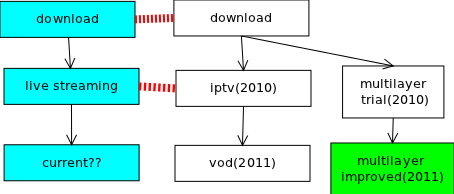
\includegraphics[width=0.6\textwidth]{../fig/version_tree.png}
	\caption{Version Tree of Real and Simulation}
	\label{fig:simu_version_tree}
\end{figure}

\textbf{Precaution}: the results obtained in this project may not 
reflect real system in every aspect(there is no red dash showing 
this kind of relationship). Nevertheless, methodology wise speaking, 
those results do provide some insights in Multilayer P2P system design.  


%\begin{itemize}
%	\item Blue: Real deployment
%	\item While: Simulation platform 
%	\item Green: This work  
%	\item Red dash: Equivalency
%\end{itemize}


\subsection{System Benchmark Test}

Before we start, system benchmark test of simulator performance
is conducted. 

%\subsubsection{Core Numbers}

Fig(\ref{fig:simu_bm_rt_core}) shows how simulator running time 
varies with different number of cores. Note that PDNS \cite{pdns}
is the distributed version of NS\cite{ns}. In this paper, we 
just run the simulation on one machine with 16 cores. The original 
configuration of the platform involves 8 cores per simulation instance. 
Leaving some system recourses for other purpose, we can only 
run one simulation at a time, which significantly lowers our 
experiment efficiency. 

\begin{figure}[htb]
\centering
	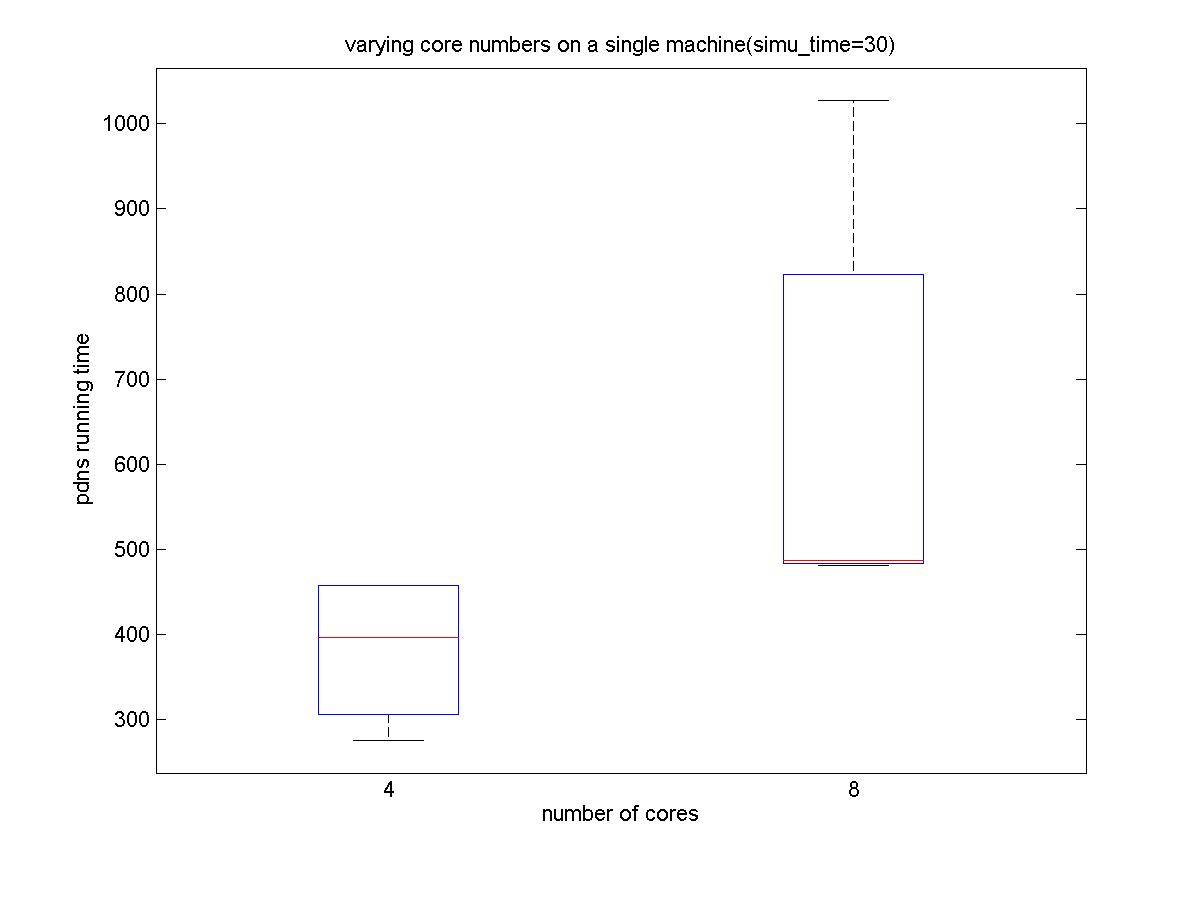
\includegraphics[width=0.7\textwidth]{../fig/runtime_vs_core.jpg}
	\caption{Running Time v.s. Number of Cores}
	\label{fig:simu_bm_rt_core}
\end{figure}

We find that, when simulation time(measured in NS seconds) is small, 
4 cores appear to be more efficient than 8 cores. Thus the following 
experiments are all issued to 4 cores to enhance our distributing level. 

%\subsubsection{Number of Nodes}

\begin{figure}[htb]
\centering
	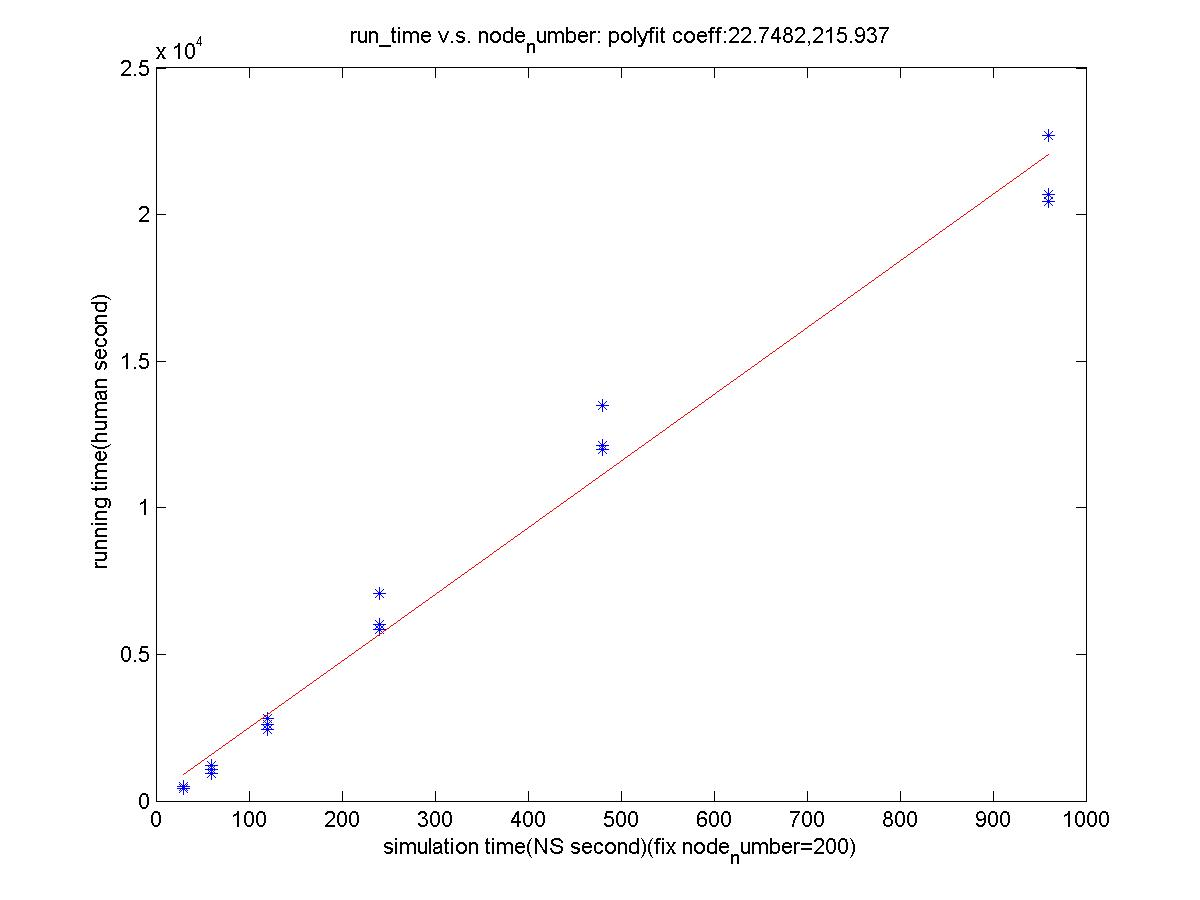
\includegraphics[width=0.7\textwidth]{../fig/runtime_vs_nodenum.jpg}
	\caption{Running Time v.s. Number of Nodes}
	\label{fig:simu_bm_rt_node}
\end{figure}

Fig(\ref{fig:simu_bm_rt_node}) shows how simulator running time 
varies with the number of nodes simulated. 
It appears to be linear. The fit parameters are given in 
the title of the plot. 

%\subsubsection{Simulation Time}

\begin{figure}[htb]
\centering
	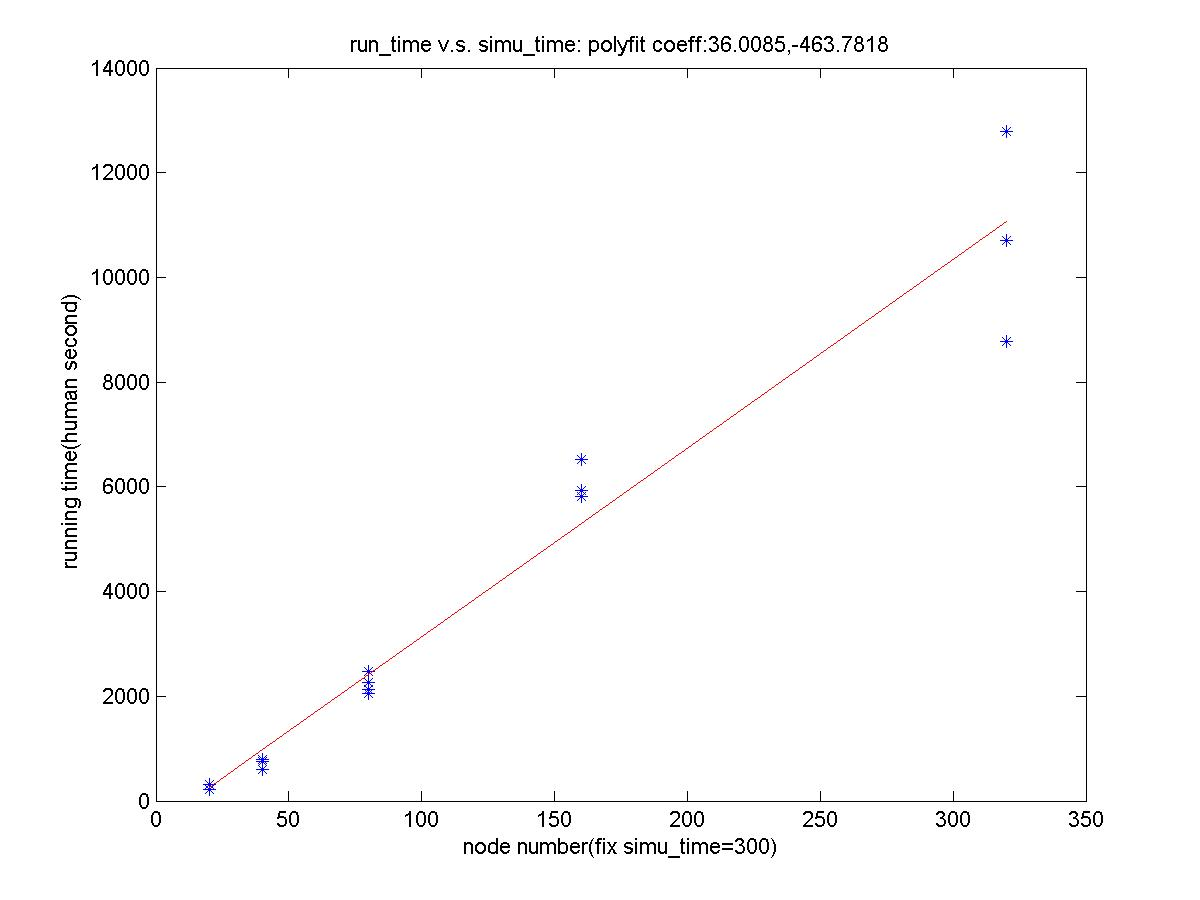
\includegraphics[width=0.7\textwidth]{../fig/runtime_vs_simutime.jpg}
	\caption{Running Time v.s. Simulation Time(NS)}
	\label{fig:simu_bm_rt_st}
\end{figure}

Fig(\ref{fig:simu_bm_rt_st}) shows how simulator running time
varies with the simulation time(in NS seconds). 

With those system test, the final parameters we choose are:
\begin{itemize}
	\item Number of Nodes: 160
	\item Simulation Time: 300 (NS seconds)
\end{itemize}

It's obviours that the number of nodes and simulation time 
is much smaller than those in a real VoD system. With those 
two configurations, the simulator can finish in about 2 hours
using 4 cores. We sacrifice some equivalency to the real system 
to make the simulation tractable. 

\subsection{Experiment Configuration}

In this study, we follow the same configuration given by 
Zheng Wen. The topology is summarized as follows:
\begin{itemize}
	\item Star like. Peers are equally divided into 4 subnets.
	Every node connects to a single central router.  
	\item Subnet parameters:
		\begin{itemize}
			\item Subnet1: down:10Mb; up:10Mb. 
			\item Subnet1: down:3Mb; up:0.5Mb. 
			\item Subnet1: down:3Mb; up:0.5Mb. 
			\item Subnet1: down:3Mb; up:0.5Mb. 
		\end{itemize}
\end{itemize}

The layer configuration is summarized as follows:
\begin{itemize}
	\item 3 Layers. 
	\item Layer parameters:
		\begin{itemize}
			\item Layer1: 256Kbit. (per piece) 
			\item Layer2: 256Kbit. (per piece) 
			\item Layer3: 512Kbit. (per piece) 
		\end{itemize}
\end{itemize}
Note that the cumulative data amount is 256Kbit, 512Kbit, and 1024Kbit. 
This is consistent with Wang's QoE study\cite{wang2011-perceptual}. Thus
we can rely on their QoE model to measure our system. 

\subsection{QoE Model Implementation}
\label{sec:simu_qoe}

In Wang's paper\cite{wang2011-perceptual}, they seek for the tradeoff
between bitrate(influenced by current layers subscribed) and discontinuity. 
They first do large amount subjective tests, and then fit the data into 
a continuous version formula, as is given in eqn(\ref{eq:mos_wang}). 
\begin{equation}
	MOS = c_1 \times d + \alpha \times (1 - e^{-b \times \lambda}) + c_2
	\label{eq:mos_wang}
\end{equation}
The parameters are $c_1=-5$, $c_2=2$, $\alpha=4$, $\lambda=0.0015$. 

In that paper, the maximum discontinuity considered is 50\%, so we 
plot the MOS curve again to give the readers a better impression of how
it looks like. See fig(\ref{fig:mos_wang}). 

\begin{figure}[htb]
\centering
	\subfigure[3D]{
	\label{fig:mos_wang_3d}
	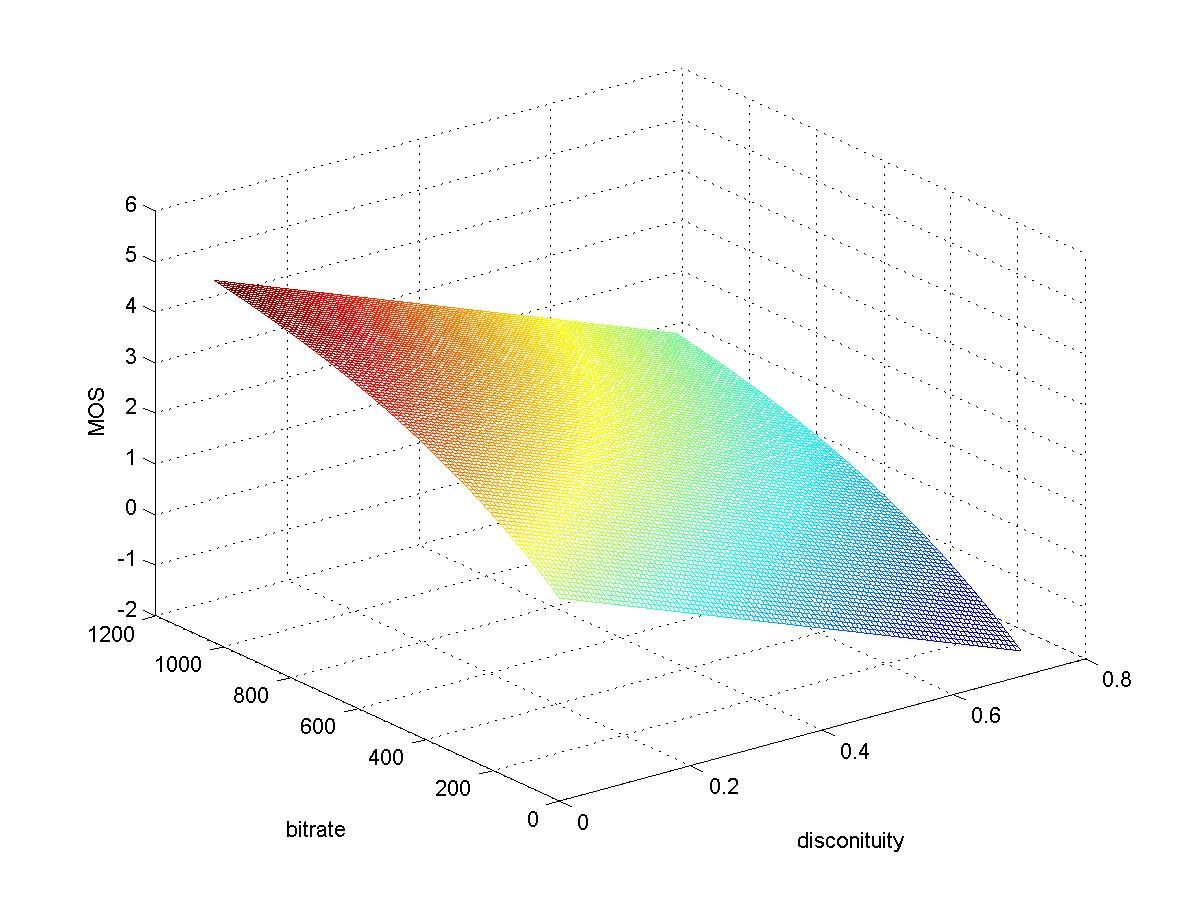
\includegraphics[width=0.45\textwidth]{../fig/bd_3d.jpg}
	}
	\subfigure[contour]{
	\label{fig:mos_wang_contour}
	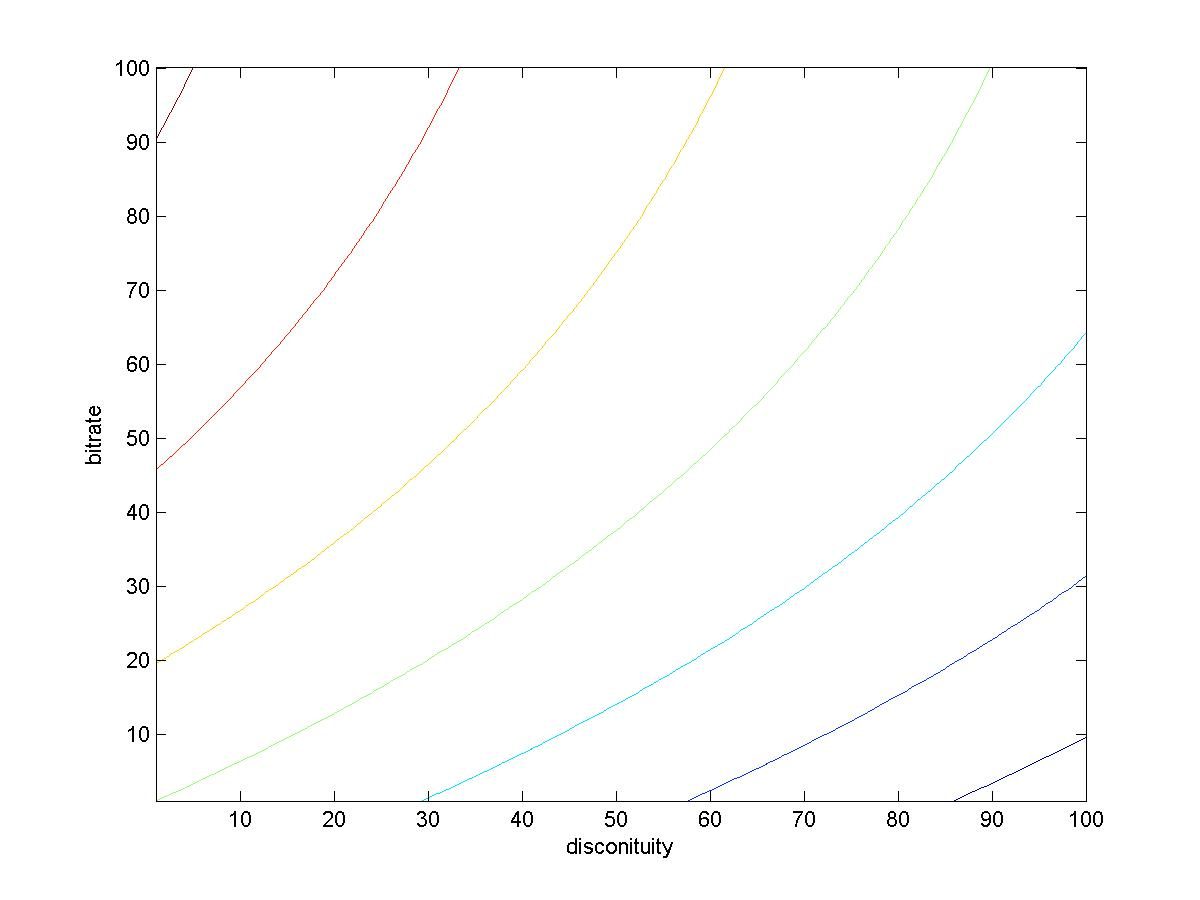
\includegraphics[width=0.45\textwidth]{../fig/bd_contour.jpg}
	}
	\caption{Conclusion, QoE and Performance}
	\label{fig:mos_wang}
\end{figure}

Fig(\ref{fig:mos_wang_3d}) is the 3D version and Fig(\ref{fig:mos_wang_contour})
is the contour version. We want to point out that by definition, MOS 
should be a score between 0 and 5. However, using this formula, we'll get
negative scores sometime. Especially when the discontinuity is 100\% and
bitrate is 0, the MOS can be as low as -3. We don't regard this case as 
a bug. On the contrary, it is reasonable to assign negative opinions. 
In our implementation of this QoE model, peers report their statistics every 
20 seconds. If the -3 score happens, that means the user is purely waiting 
in the whole 20 seconds, which causes a negative opinion naturally. 
Our system should work towards reducing this kind of disturbance. 

\subsection{Baseline Test}
\label{sec:simu_base}

In this section, we evaluate the baseline using the QoE records 
reported by peers. We compute MOS using eqn(\ref{eq:mos_wang}),
and take the average. 

Fig(\ref{fig:simu_base_qoe_st}) shows the result when total simulation 
time varies from 30 NS seconds to 960 NS seconds. It's interesting that
with the increase of simulation time, the QoE gets improved, and the 
boxplot shows the statistics of 5 simulations with the same 
configuration. This means the improvement is statistically significant. 

\begin{figure}[htb]
\centering
	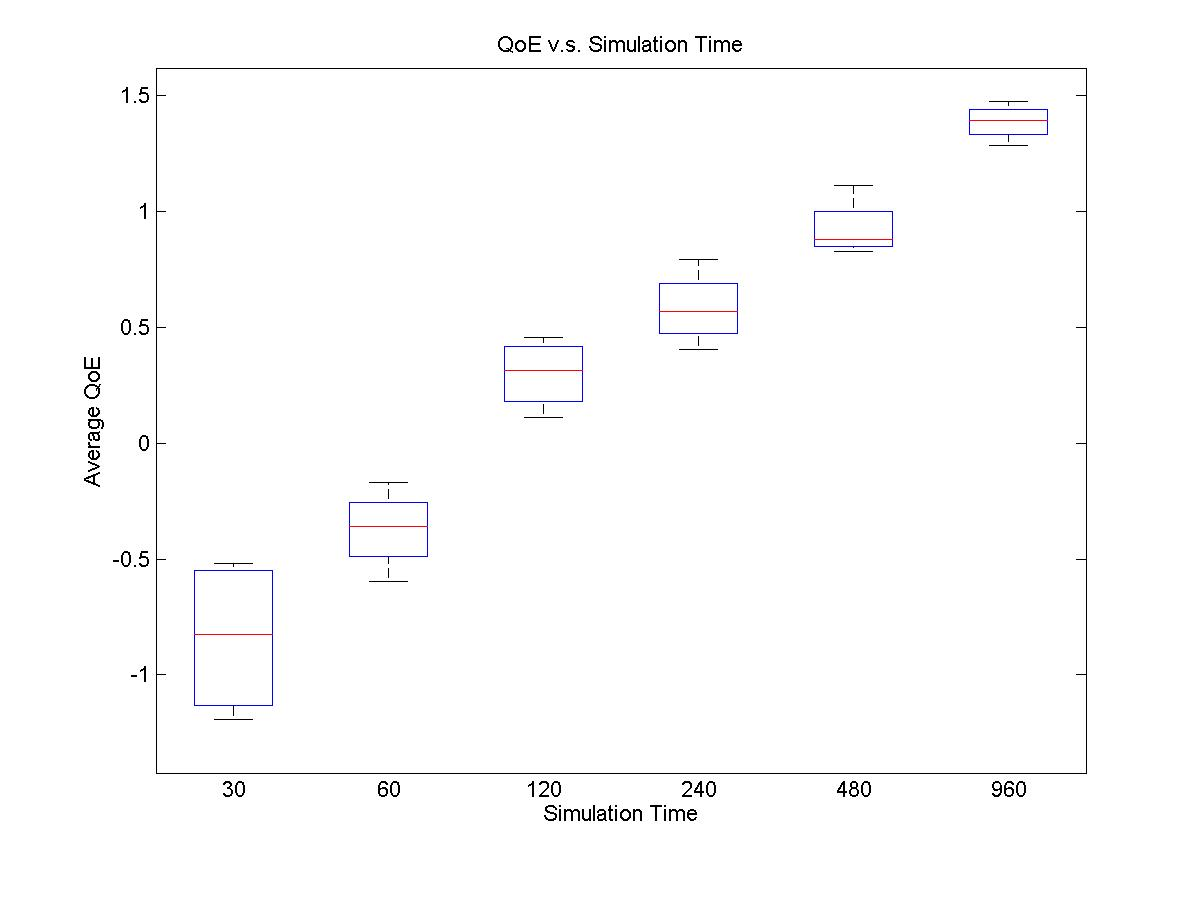
\includegraphics[width=0.7\textwidth]{../fig/simutime_qoe.jpg}
	\caption{QoE v.s. Simulation Time}
	\label{fig:simu_base_qoe_st}
\end{figure}

By examing the detailed trace file, we find that there are many 
negative opinions at the beginning of those simulation. Later after
about 100 NS seconds, the reported MOS gets better and better. It
makes sense that the system needs some bootstraping time, when 
all of the peers lack chunks. They can not help each other efficiently
during this time. 

We eliminate those negative records and make the boxplot again. See 
Fig(\ref{fig:simu_base_qoenonneg_st}). This figure verifies our 
conjecture. The last two boxes stand for 480s and 960s simulation time. 
There is little difference in mean within this range. Longer simulation time
just makes the variance smaller. To explain, after some bootstraping period, 
the system approaches steady state and the average opinions become 
nearly a constant. The first box seems an outlier. This is because peers are
joining the system gradually at that time. The number of reported records
are very small. Only those peers connected directly to the source can 
get something to playback. Others all get negative opinions. By eliminating 
the negative opinions, the resultant score is very high. 

\begin{figure}[htb]
\centering
	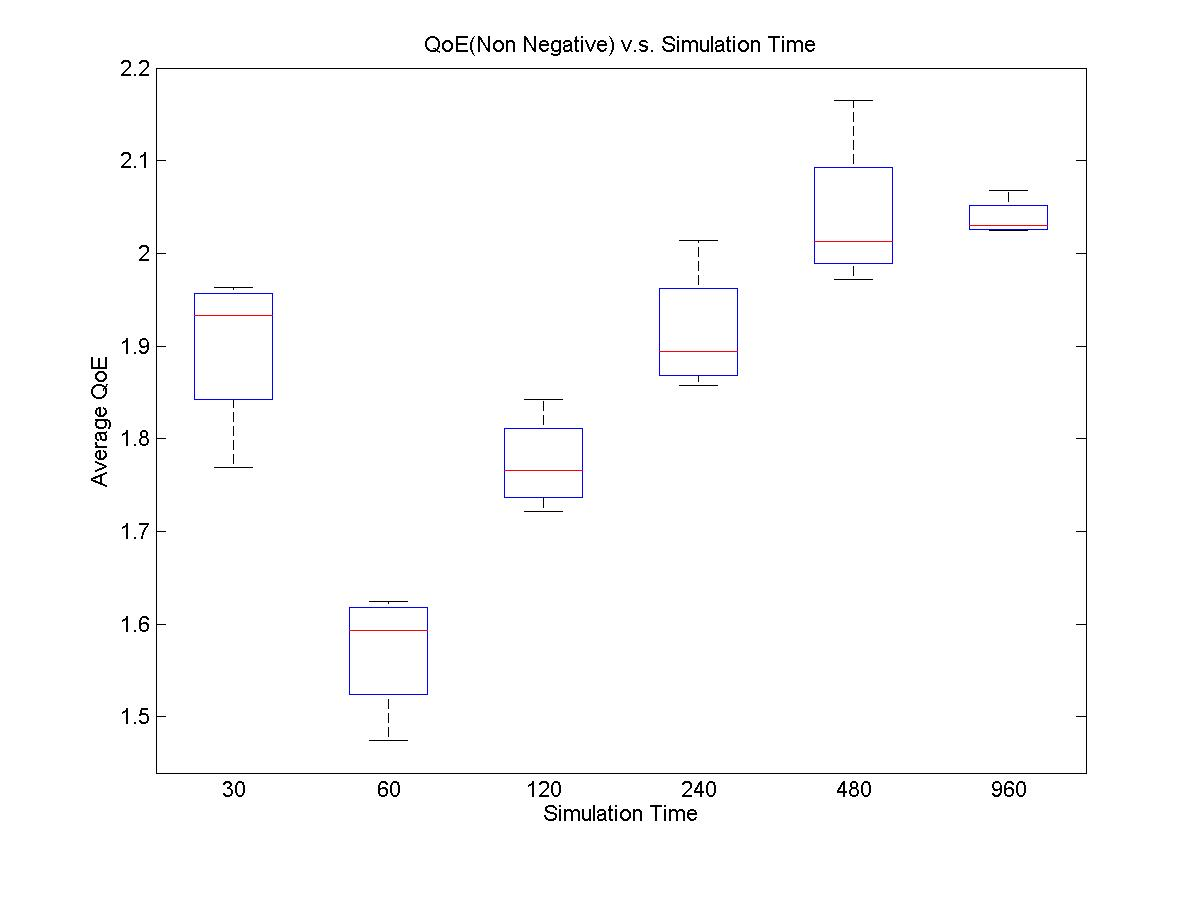
\includegraphics[width=0.7\textwidth]{../fig/simutime_qoe_nonneg.jpg}
	\caption{QoE(nonneg) v.s. Simulation Time}
	\label{fig:simu_base_qoenonneg_st}
\end{figure}



%
%\begin{itemize}
%      \item     $'count\_mr' => 3749$
%      \item     $'count\_mr\_nonneg' => 2601$
%      \item     $'avg\_qoe' => '0.871540677419684'$
%      \item     $'avg\_qoe\_nonneg' => '2.01996612593628'$
%      \item     $'node\_num' => '160'$
%      \item     $'simu\_time' => '480'$
%      \item     $'core\_num' => '4'$
%      \item     $'task\_duration' => 8399$
%      \item     $'pdns\_duration' => 8302$
%\end{itemize}

Next, we pick a sample run out of all these baseline simulations. 
The global parameters and statistics are: 
simulation time is 480s; number of nodes is 160;
number of QoE reports is 3749; number of nonnegative QoE reports is 2601;
average QoE socre is 0.87; the nonnegative version of average QoE score is 
2.02. 

\begin{figure}[htb]
\centering
	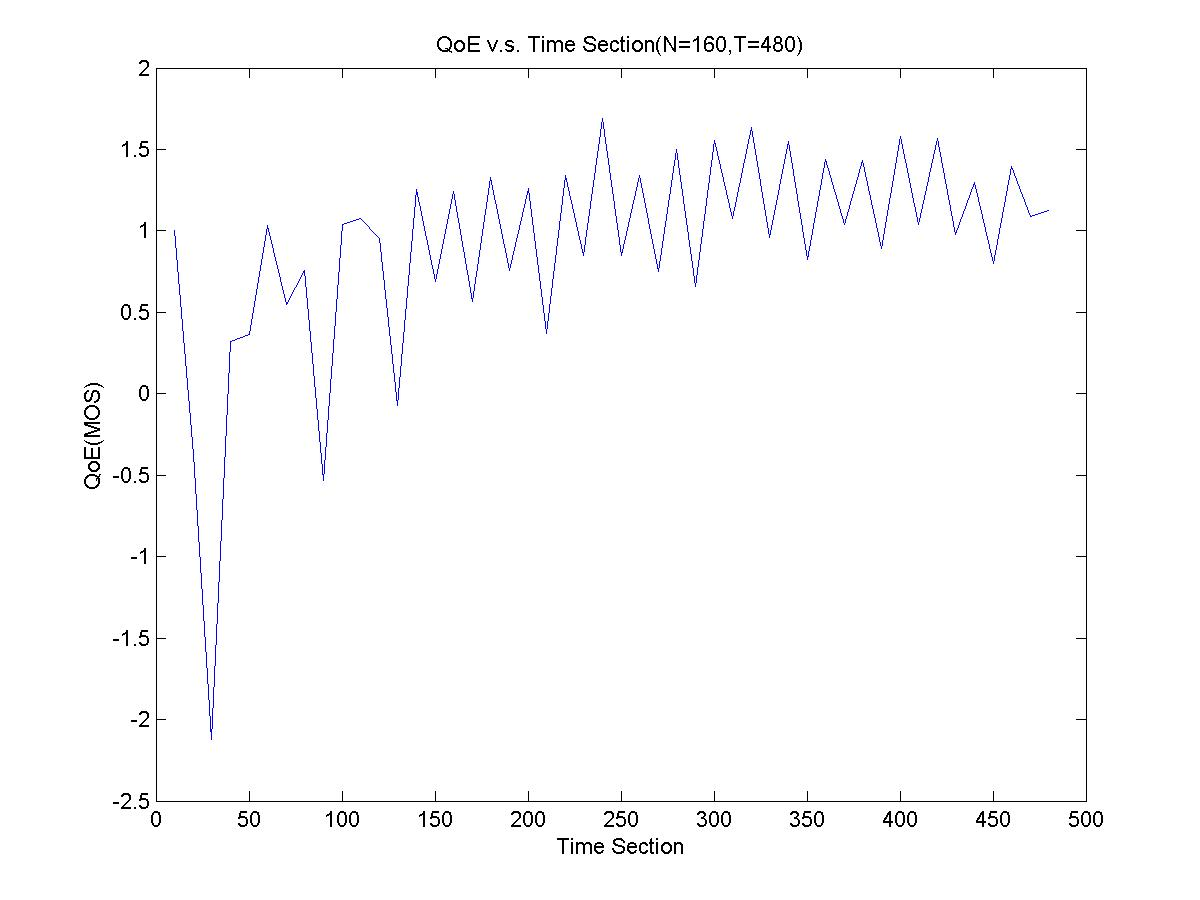
\includegraphics[width=0.7\textwidth]{../fig/time_qoe.jpg}
	\caption{QoE Varies with Current System Time}
	\label{fig:simu_base_qoe_vary}
\end{figure}


Fig(\ref{fig:simu_base_qoe_vary}) shows how QoE varies with curret time section. 
We can see the per section averaged QoE gets higher and higher in 
the first 150 seconds. After that, the section averaged QoE becomes steady. 
This again proves our bootstraping conjecture. 


\begin{figure}[htb]
\centering
	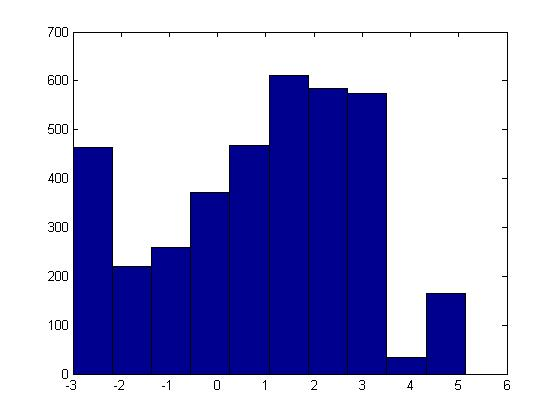
\includegraphics[width=0.7\textwidth]{../fig/qoe_hist.jpg}
	\caption{Histogram of QoE Distribution}
	\label{fig:simu_base_qoe_distri}
\end{figure}

Fig(\ref{fig:simu_base_qoe_distri}) shows the historgram of QoE reports
from this sample run. We can conclude that, some powerful peers can get 
full 5 score experiene, whereas large amount of peers report negative scores.
Our future improvements should mitigate this part(purely buffer for 
20 seconds and play nothing). 

\subsection{Chunk Selection Architecture Reconstruction}
\label{sec:arch}

In this section, we modify the original architecture to make
it more clear and unified. This helps us develop strategies 
on this architecture later. 

Original design separates chunk selection and peer selection. 
It is shown in Fig(\ref{fig:simu_arch_orig}). 

\begin{figure}[htb]
\centering
	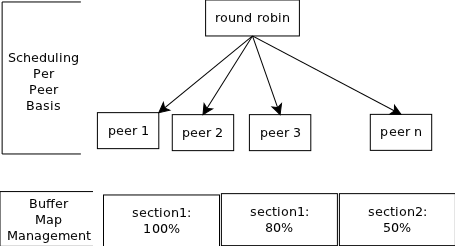
\includegraphics[width=0.7\textwidth]{../fig/arch_orig.png}
	\caption{Original Architecture}
	\label{fig:simu_arch_orig}
\end{figure}

In this design, every peer is considered in a round robin fashion. 
After one neighbour is chosen, this peer selects chunks according to 
a three section based strategy. After one section is filled up to a 
certain ratio, the peer
will consider the next section. Chunks in the same section are selected 
randomly. In our multilayer situation, layers are considered from lower ones
to higher ones. That is, after the peer get 50\% of the 3rd section, 
it will start to to fill the next higher layer. 
In order to reduce the network burden, peers are constrained to fetch chunks
from no more than 20 neighbours simultaneously. 

\begin{figure}[htb]
\centering
	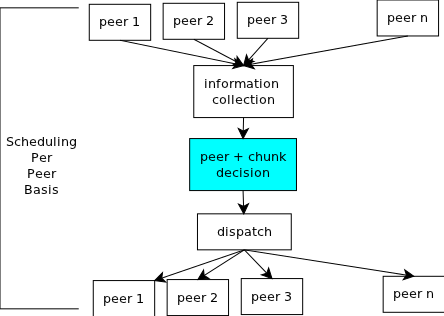
\includegraphics[width=0.7\textwidth]{../fig/arch_improved.png}
	\caption{Improved Architecture}
	\label{fig:simu_arch_improv}
\end{figure}

The improved architecture is illustrated in Fig(\ref{fig:simu_arch_improv}). 
To make our decision more rationale and make the architecture clear,
we collect all information first, and do peer selection and chunk selection 
together. 

In this version, we adopt a very simple strategy, as is used in PALS
\cite{rejaie2003pals}. This strategy makes decision on a chunk basis. 
It first consider base layer chunks and then moves to enhancement layers. 
In one layer, the chunks closer to playback points are considered first. 
The overall picture is like a snake-shaped move on the 2 dimension buffer
map. Fig(\ref{fig:simu_stg_pals}) illustrates this strategy. 
If there are more than one peers available for one chunk, we just randomly 
choose one peer. 

\begin{figure}[htb]
\centering
	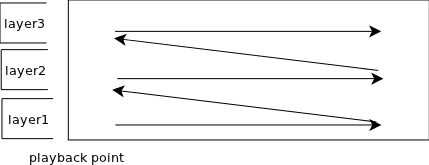
\includegraphics[width=0.7\textwidth]{../fig/pals_like.png}
	\caption{PALS Style Chunk Selection}
	\label{fig:simu_stg_pals}
\end{figure}

After each modification, we evaluate the result from two aspects:
\begin{itemize}
	\item QoE. The formula is given in eqn(\ref{eq:mos_wang}). 
	In our study, we didn't make any aggressive strategies like
	scheduling all requests to the server. So we don't subtract server's
	contribution from this metric intentionally. Another reason is, 
	in the underlying overlay construction(which is not modified in 
	this study), the server is treated as a normal peer. Not all peers
	can turn to server for help when the lack chunks. 
	\item Performance. Another important thing we care is the performance
	of simulator. This kind of packet level simulation is very time consuming. 
	One iteration of strategies calls for several hours of running typically. 
	In order to fulfil a short-term project, we can not make strategies of 
	high time complexity. What's more, the running time of simulator 
	reflects the computation resource consumption in real deployments. 
	User experience will degrade if their player consumes extra large
	amount of resources, to limit other process. 
\end{itemize}

The result of modification in this section is:
\begin{itemize}
	\item QoE: 0.7 $\rightarrow$ 3.3
	\item Performance: nearly doubled. 
\end{itemize}


\subsection{Priority Based Upgrade}
\label{sec:priority}

In this section, we do more engineering upgrades. 
We abstract the chunk selection strategy using a priority table. 
One sample table with window size equal to 5 is given in 
Table(\ref{tbl:sample_priority}). This table is equivalent to 
PALS. 

\begin{table}[htb]
\centering
\caption{A Sample Priority Table with Window Size = 5}
\label{tbl:sample_priority}
	\begin{tabular}{|c|ccccc|}
	\hline
	 & t1 & t2 & t3 & t4 & t5 \\
	 \hline
	layer3 & 11 & 12 & 13 & 14 & 15 \\
	layer2 & 6 & 7 & 8 & 9 & 10 \\
	layer1 & 1 & 2 & 3 & 4 & 5 \\
	\hline
	\end{tabular}
\end{table}

Further investigation on optimal priority table can be done 
easily in this framework. Result of this modification is:
\begin{itemize}
	\item QoE: nearly the same. 
	\item Performance: decrease slightly. 
\end{itemize}


\subsection{Scalable Window Size}

After previous upgrades, we examine the trace files from 
several simulations. From the trace, we find many powerful peeers can get full 
3 layers in the whole window(60 seconds, 3 layers). 
The restriction on window size is a special desgin of video streaming, 
no matter live or VoD. This is because chunks very far from 
playback point is not of high interest to the peer. Every peer 
only needs to store enough chunks in the buffer to guarantee 
smooth playback. However, there is a side effect. Capable peers
who are playing the early part can not help others who are 
playing the later part. Thus we want to give those peers a chance to 
help others. This is the rationale behind scalable window size. 

\begin{table}[htb]
\centering
\caption{A Sample Priority Table with Window Size = 5+5}
\label{tbl:priority_scalable}
	\begin{tabular}{|c|ccccc|c|}
	\hline
	 & t1 & t2 & t3 & t4 & t5 & t6-t10 \\
	 \hline
	layer3 & 11 & 12 & 13 & 14 & 15 & ...\\
	layer2 & 6 & 7 & 8 & 9 & 10 & ... \\
	layer1 & 1 & 2 & 3 & 4 & 5  & ...\\
	\hline
	\end{tabular}
\end{table}

Table(\ref{tbl:priority_scalable}) illustrates a scaled 
window with the size doubled. Using this table, less capable 
peers will act as they are using table(\ref{tbl:sample_priority}). 
For those powerful peers, after they finish the first section, as 
is in table(\ref{tbl:priority_scalable}), they can move to the second
section. This is the simplest illustration of the idea of scalable 
window size. Ideally, the window size should be computed 
on recipient of heartbeat message. When a peer updates the 
network connection measurements, it can compute a proper window 
size based on those data. Last but not least, the priority table 
should be recomputed if the window size changes. 

In this version, we fill the second section of the window using 
the same strategy as used for the first section. The result is:
\begin{itemize}
	\item QoE is improved a little. 
	\item Performance degrades sharply. 
\end{itemize}


\subsection{Performance Optimization}
\label{sec:perf}

After last experiment, one simulation needs about 4.5 hours to complete. 
This is really time consuming. In order to do more iterations, we 
try to optimize the simulator performance right away. 
At first, optimization described in this section only aims at 
the performance of simulator. However, it turns out the QoE is 
also improved. We'll talk about this phenomenon in conclusion section. 

\begin{figure}[htb]
\centering
	\subfigure{
	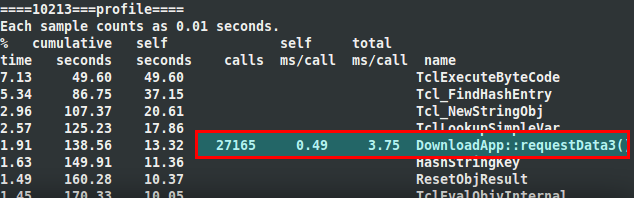
\includegraphics[width=0.6\textwidth]{../fig/gprof1.png}
	} \\
	\subfigure{
	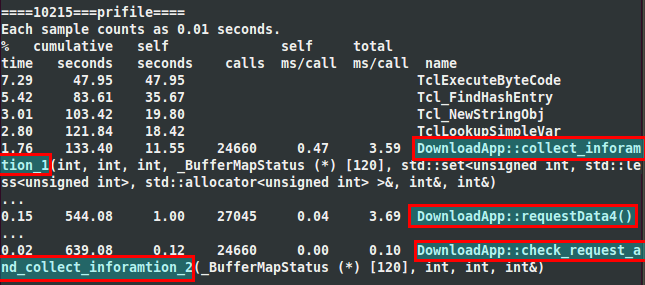
\includegraphics[width=0.6\textwidth]{../fig/gprof2.png}
	}
	\caption{GNU Profile, Output}
	\label{fig:simu_perf_gprof}
\end{figure}

Fig(\ref{fig:simu_perf_gprof}) shows two screenshots of the 
output of 'gprof'. We first locate the most time consuming part
that we can control. It turns out to be the 'requestData3()' function, 
which implements the strategy mentioned in last section. 
We then separate some sub functions from this one and find that
the information collection is most time consuming. Note that 
we do not send probes to collect information. Instead, peer information
is updated on recipient of periodical notification message. 
The information collection sub function only iterates over some 
map structures and fill the availability information into 
one unified 2D buffer map. 

According to the analysis of the profile, we optimized those iteration 
process. For more details, please refer to the code repository 
of this project. Difference can be found between the following 
two commitments:
\begin{Verbatim}
b45038404d8970c8ee1654d9bdbb10703432b8cd
5d3aabdb1546d88da6e7a026d2d1fe67b04ad2f1
\end{Verbatim}

Result of the optimization is:
\begin{itemize}
	\item QoE: improved a little. 
	\item Performance: 4.5h $\rightarrow$ 3.5h. 
\end{itemize}

Note that this is not the end of the performance optimization. 
One of the possible directions is to optimize the sampling 
method using a reservoir\cite{vitter1985-random-reservoir}. 
However, this optimization is conducted with the knowledge 
that we'll only random select one peer if there are multiple peers
available for one chunk. This kind of optimization is too aggressive
and will limit the design space of strategies, so we don't do 
them in this research version. Designers can make notes 
and do this kind of optimization when all strategies are fixed 
in a real release version. 

\subsection{Introduce Randomness in Second Window Section}

Due to time issue, our last trial based on the already established 
mechanism is to introduce randomness in second window section. 
As is known, randomness is a good property in the sense 
that it helps the system to spread chunks uniformly. The first window
section is scheduled using a snake-shaped priority, this design considers
user-perceived experience. However, the second window section is for
those powerful peers. Those chunks are not hurry for playback. Thus 
we make the second section of the priority table randomly initialized. 
Every peer will have different priority table. 

The result is:
\begin{itemize}
	\item QoE: get worse. 
	\item Performance: get worse. 
\end{itemize}

\subsection{Conclusion of the Case Study}
\label{sec:simu_con}

In this section we put together the result of 6 big versions. 
See Fig(\ref{fig:simu_con}). In terms of QoE, version 2 improves
a lot from baseline. After that, there are not so much difference 
in QoE. In terms of simulator performance, all modified versions 
are slower. The slowest version is the scalable window one. From 
the plot, we know our performance optimization really helps to 
reduce running time. 

\begin{figure}[htb]
\centering
	\subfigure[qoe]{
	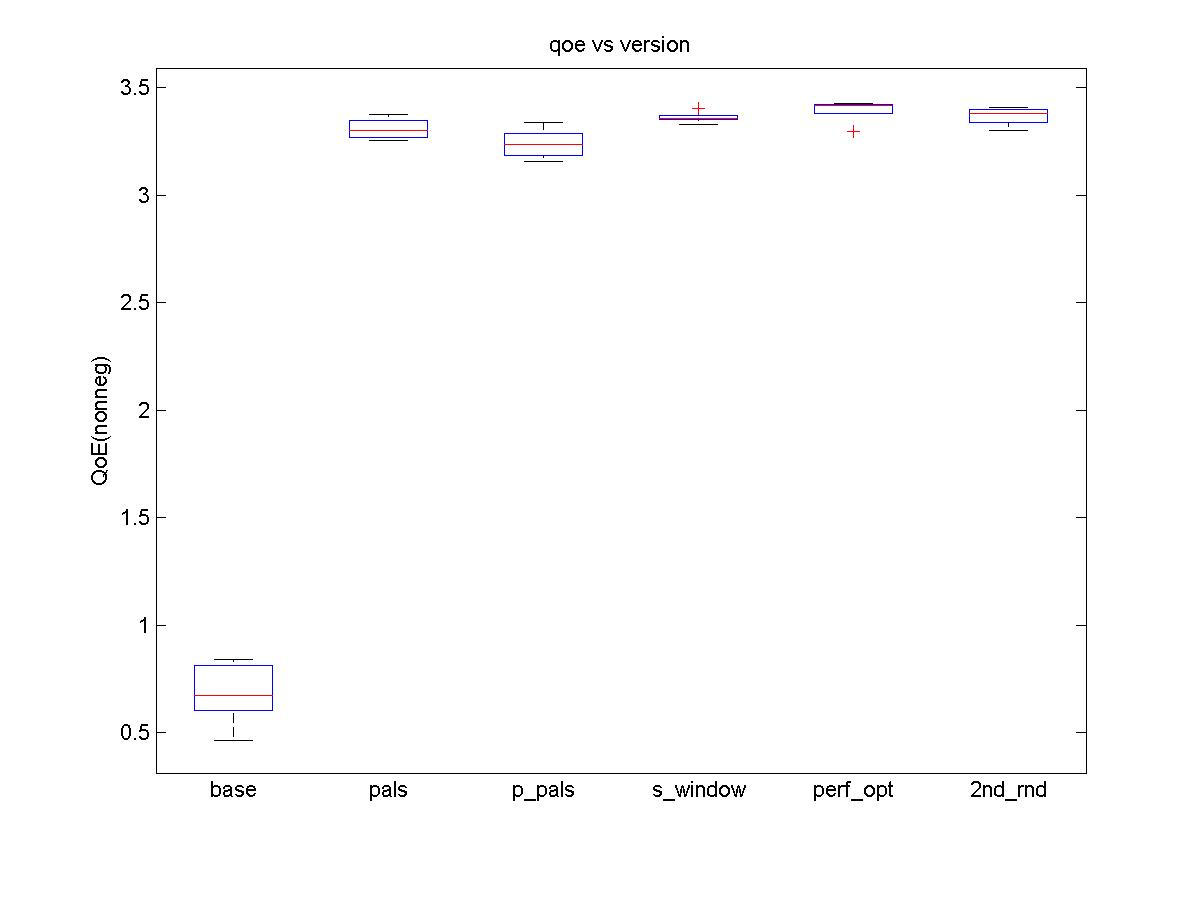
\includegraphics[width=0.45\textwidth]{../fig/con_qoe_version_all.jpg}
	}
	\subfigure[time]{
	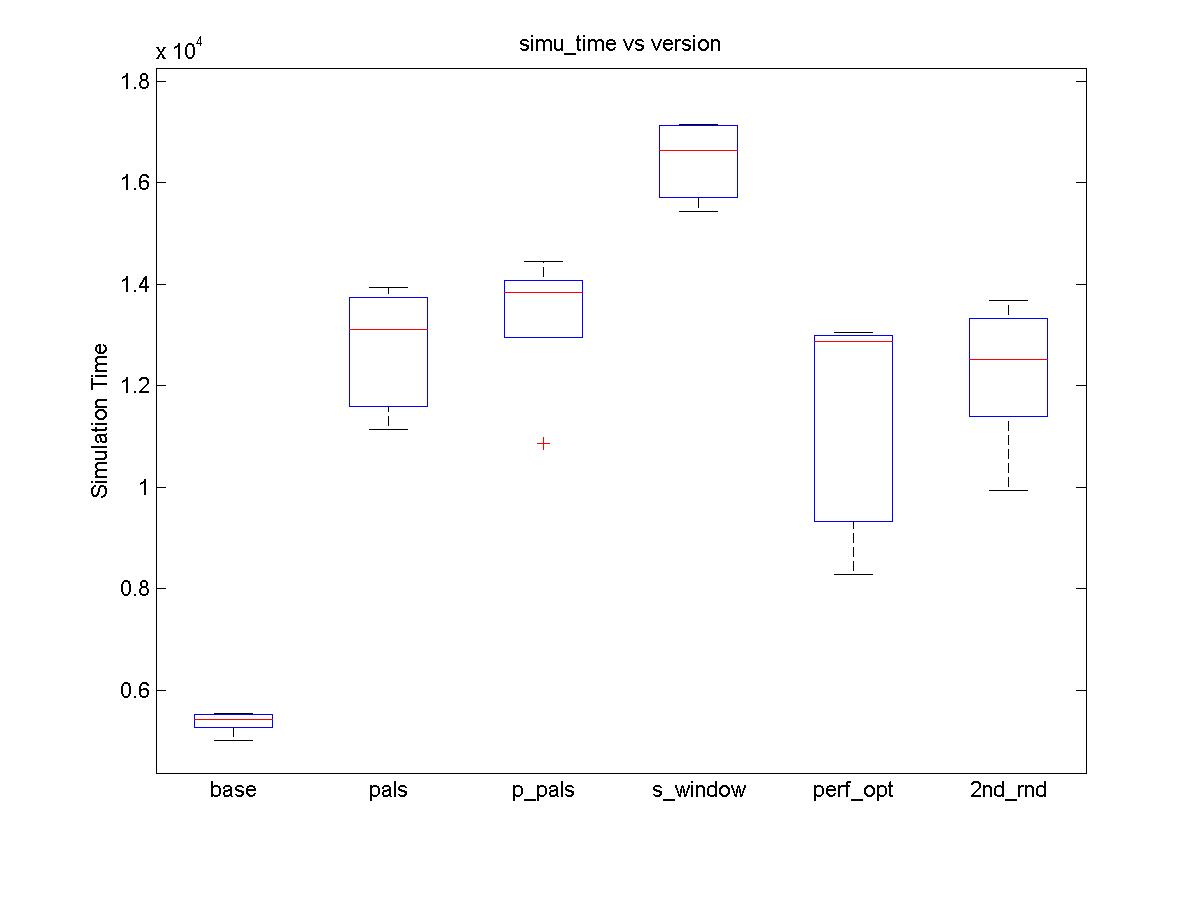
\includegraphics[width=0.45\textwidth]{../fig/con_time_version_all.jpg}
	}
	\caption{Conclusion, QoE and Performance}
	\label{fig:simu_con}
\end{figure}

Fig(\ref{fig:simu_con_detail}) gives a closer look at the 5 modified versions. 
The most interesting observation is the difference before and after 
performance optimization. Note that in section(\ref{sec:perf}), 
we did nothing about strategy. It is simply equivalent code reconstruction.
However, while we observe better performace of the simulator, we also 
find the QoE is improved a little. From the box plot, this improvement 
seems statistically significant(there are two ourliers). 


\begin{figure}[htb]
\centering
	\subfigure[qoe]{
	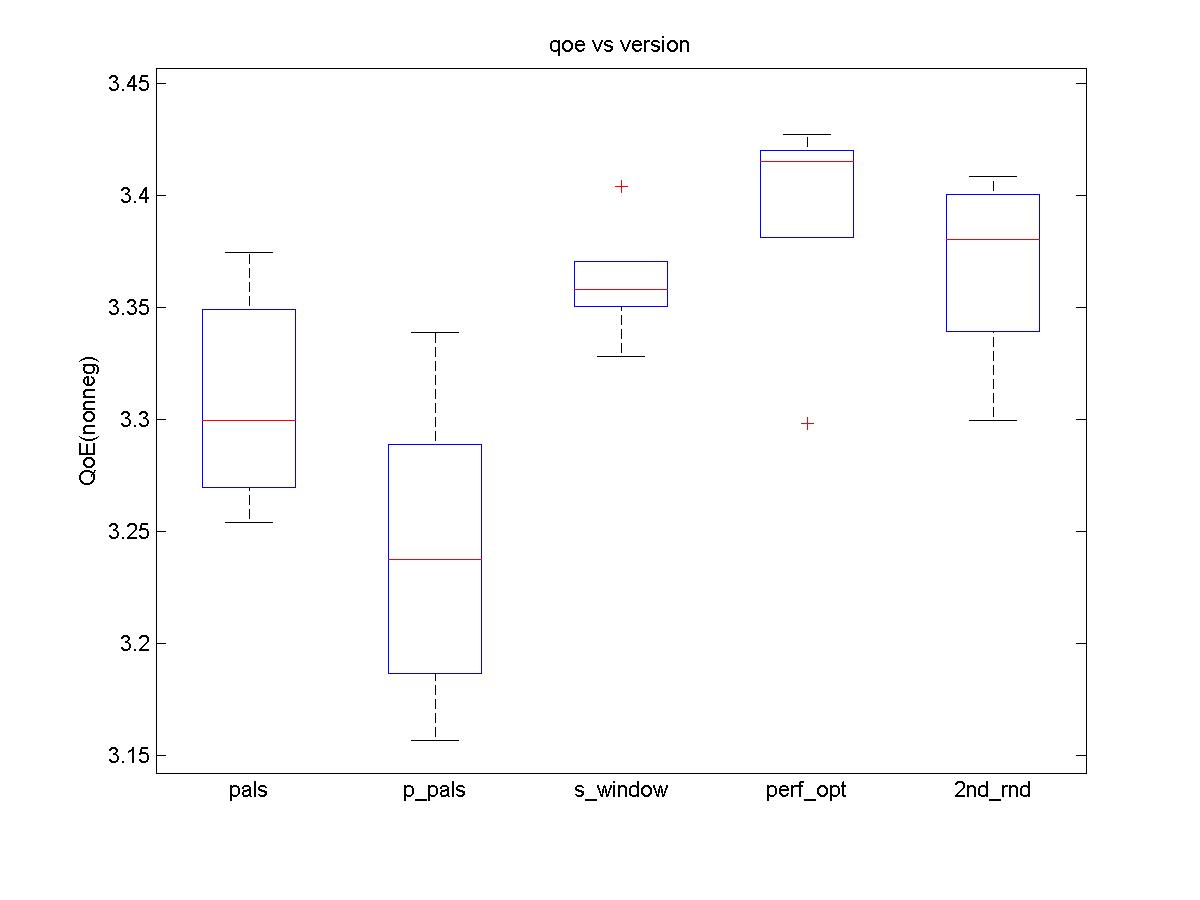
\includegraphics[width=0.45\textwidth]{../fig/con_qoe_version_part.jpg}
	}
	\subfigure[time]{
	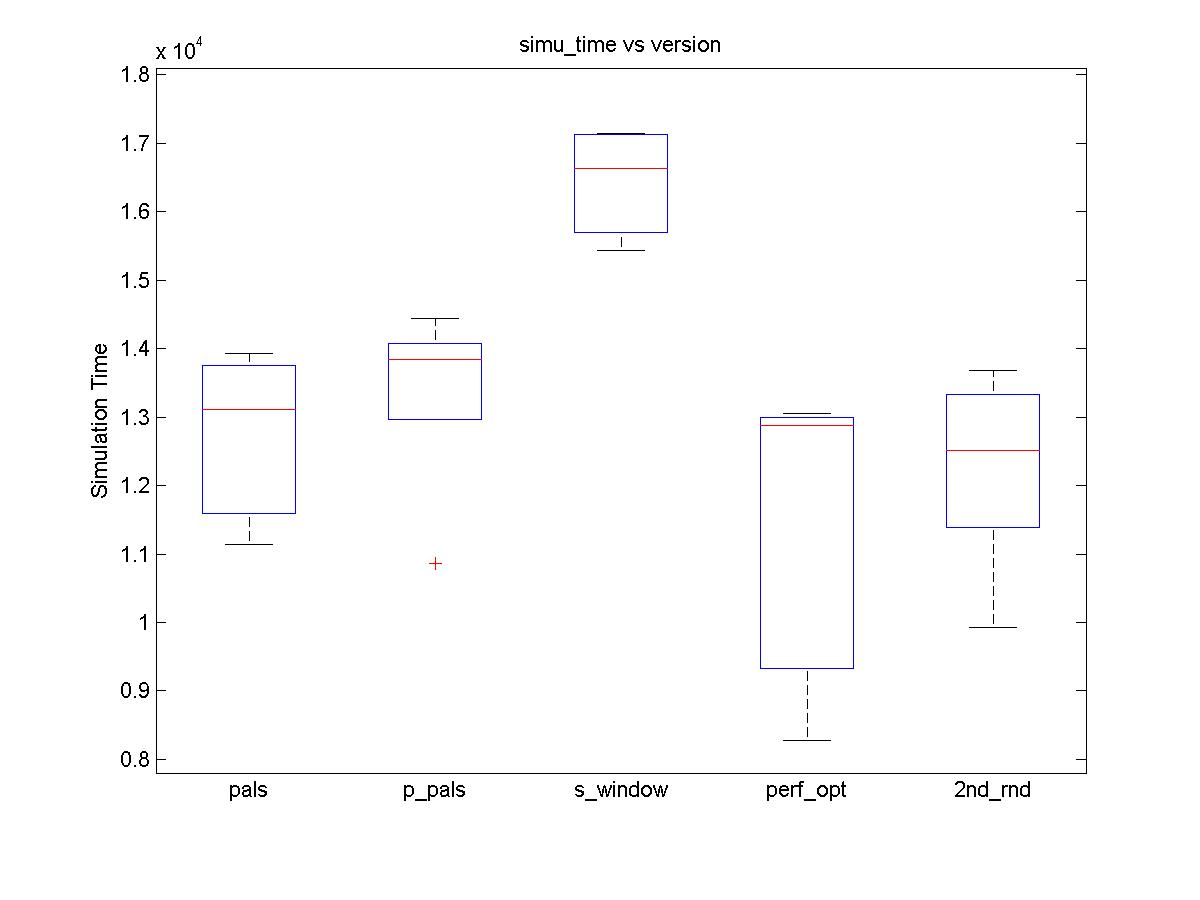
\includegraphics[width=0.45\textwidth]{../fig/con_time_version_part.jpg}
	}
	\caption{Conclusion, QoE and Performance}
	\label{fig:simu_con_detail}
\end{figure}

Similar phenomena have been observed in our other VoD simulations using 
the same series ASTRI platform\cite{huang2010simulation}. When the server 
is idle, the results tends to be better. Just like in our experiment, after 
performance optimization, the computation burden is lowered, thus we see 
better results. One conjecture is that this phenomenon is due to underlying 
timing facilities, either NS\cite{ns,pdns} layer or the p2p simulator 
layer\cite{huang2010simulation}. The verification of this point is
left as future work. 


\section{Conclusion}
\label{sec:conclusion}

Here we conclude two pieces of experience from this study:
	\begin{itemize}
		\item Engineering approach v.s. academic approach:
		where is the biggest cake? From section(\ref{sec:simu_con}), 
		we see the most significant improvement lies in the first 
		engineering upgrade. Although the modification itself reads simple, 
		it makes the strategy framework more clear. Upon this framework, 
		one simplest PALS like strategy achieves very good result. 
		By examining the simulator carefully, we believe more engineering 
		optimization can be found. Without an ideal underlying 
		platform, the verification of algorithms on it is questionable. 
		At same time, the benefit we tried exhaustively to get 
		using better strategies may come easier with some engineering 
		upgrades. 
		\item Time distribution of this project:
			\begin{itemize}
				\item 70\%, literature survey.(30+ papers) 
				\item 15\%, environment setup, bugfix of the platform. 
				\item 5\%, first unified version(QoE:0.7$\rightarrow$3.3, 
				biggest improvement in this study)
				\item 10\%, scalable window, performance optimization, random 
				2nd section. (little outcome)
			\end{itemize}
		Sometimes we try very hard, to get little outcome. Sometimes, 
		ideas flash through our minds, and suddenly we get significant 
		achievements. 
	\end{itemize}

%\begin{itemize}
%	\item 6 big versions / 240 runs. 
%	\item Auxilary Scripts:
%	\begin{itemize}
%	\item .sh:298 lines
%	\item .pl:791  lines
%	\item .m:133 lines
%	\end{itemize}
%	\item Simulation Code Difference:	
%	\begin{itemize}
%		\item download\_agent.cc: 1940 lines
%		\item download\_agent.h: 301 lines
%		\item labtesting.tcl: 84 lines
%	\end{itemize}
%\end{itemize}


\section{Future Works}
\label{sec:future}

%Here we list some potential research topics in an adaptive video streaming 
%system:
%\begin{itemize}
%	\item 
%\end{itemize} 

For multilayer P2P VoD system, we list some potential research topics:
\begin{itemize}
	\item Degree composition and decomposition. 
	\item If we use the framework given in section(\ref{sec:priority}), 
	what's the optimal priority table. In order to achieve QoE aware design, 
	models like \cite{wang2011-perceptual} should be considered. Due to 
	time limit, we haven't deducted the optimal table in this study. 
	\item As for the simulator, how to explain the relationship between 
	QoE and simulator performance. Theoretically speaking, QoE should only 
	depend on strategies and irrelevant of simulator performance. 
\end{itemize}
(Not complete list. See my homepage for further amendments)

\question

\section*{Acknowledgements}
\addcontentsline{toc}{section}{Acknowledgements}

The author would like to thank course instructor of IERG5270, Professor
DM Chiu, and course TA Tom Fu. The inspiring discussion with professor 
Wing Lau is very helpful. That helps the author find related works 
in the context of IP multicast. The support from ASTRI\cite{astri} is also important, 
which helps us get a better understanding of the commercial deployment
of a multilayer P2P VoD system. The baseline platform is developed 
by Zheng Wen, HKU. Special thanks to those coding. 


\pagebreak
\section*{Appendix}
\addcontentsline{toc}{section}{Appendix}


%\pagebreak
\addcontentsline{toc}{section}{References}
\input{gen_bib.bbl}


\end{document}